%\documentclass[UTF8]{ctexart} % use larger type; default would be 10pt
\documentclass[a4paper]{article}
\usepackage{xeCJK}
%\usepackage[utf8]{inputenc} % set input encoding (not needed with XeLaTeX)

%%% Examples of Article customizations
% These packages are optional, depending whether you want the features they provide.
% See the LaTeX Companion or other references for full information.

%%% PAGE DIMENSIONS
\usepackage{geometry} % to change the page dimensions
\geometry{a4paper} % or letterpaper (US) or a5paper or....
\geometry{margin=1in} % for example, change the margins to 2 inches all round
% \geometry{landscape} % set up the page for landscape
%   read geometry.pdf for detailed page layout information

\usepackage{graphicx} % support the \includegraphics command and options

% \usepackage[parfill]{parskip} % Activate to begin paragraphs with an empty line rather than an indent

%%% PACKAGES
\usepackage{booktabs} % for much better looking tables
\usepackage{array} % for better arrays (eg matrices) in maths
\usepackage{paralist} % very flexible & customisable lists (eg. enumerate/itemize, etc.)
\usepackage{verbatim} % adds environment for commenting out blocks of text & for better verbatim
\usepackage{subfig} % make it possible to include more than one captioned figure/table in a single float
% These packages are all incorporated in the memoir class to one degree or another...

%%% HEADERS & FOOTERS
\usepackage{fancyhdr} % This should be set AFTER setting up the page geometry
\pagestyle{fancy} % options: empty , plain , fancy
\renewcommand{\headrulewidth}{0pt} % customise the layout...
\lhead{}\chead{}\rhead{}
\lfoot{}\cfoot{\thepage}\rfoot{}

%%% SECTION TITLE APPEARANCE
\usepackage{sectsty}
\allsectionsfont{\sffamily\mdseries\upshape} % (See the fntguide.pdf for font help)
% (This matches ConTeXt defaults)

%%% ToC (table of contents) APPEARANCE
\usepackage[nottoc,notlof,notlot]{tocbibind} % Put the bibliography in the ToC
\usepackage[titles,subfigure]{tocloft} % Alter the style of the Table of Contents
\renewcommand{\cftsecfont}{\rmfamily\mdseries\upshape}
\renewcommand{\cftsecpagefont}{\rmfamily\mdseries\upshape} % No bold!

%%% END Article customizations

%%% The "real" document content comes below...

\setlength{\parindent}{0pt}
\usepackage{physics}
\usepackage{amsmath}
%\usepackage{symbols}
\usepackage{AMSFonts}
\usepackage{bm}
%\usepackage{eucal}
\usepackage{mathrsfs}
\usepackage{amssymb}
\usepackage{float}
\usepackage{multicol}
\usepackage{abstract}
\usepackage{empheq}
\usepackage{extarrows}
\usepackage{textcomp}
\usepackage{fontspec}
\usepackage{braket}
\usepackage{siunitx}
\sisetup{
	separate-uncertainty = true,
	inter-unit-product = \ensuremath{{}\cdot{}}
}
\usepackage{mhchem}
\usepackage{hyperref}
\hypersetup{
	colorlinks=true,
	linkcolor=black,
	filecolor=magenta,      
	urlcolor=cyan,
}

\DeclareMathOperator{\p}{\prime}
\DeclareMathOperator{\ti}{\times}
\DeclareMathOperator{\intinf}{\int_0^\infty}
\DeclareMathOperator{\intdinf}{\int_{-\infty}^\infty}
\DeclareMathOperator{\intzpi}{\int_0^\pi}
\DeclareMathOperator{\intztpi}{\int_0^{2\pi}}
\DeclareMathOperator{\sumninf}{\sum_{n=1}^{\infty}}
\DeclareMathOperator{\sumninfz}{\sum_{n=0}^\infty}
\DeclareMathOperator{\sumiinf}{\sum_{i=1}^{\infty}}
\DeclareMathOperator{\sumiinfz}{\sum_{i=0}^\infty}
\DeclareMathOperator{\sumkinf}{\sum_{k=1}^{\infty}}
\DeclareMathOperator{\sumkinfz}{\sum_{k=0}^\infty}
\DeclareMathOperator{\e}{\mathrm{e}}
\DeclareMathOperator{\I}{\mathrm{i}}
\DeclareMathOperator{\Arg}{\mathrm{Arg}}
\DeclareMathOperator{\ra}{\rightarrow}
\DeclareMathOperator{\llra}{\longleftrightarrow}
\DeclareMathOperator{\lra}{\longrightarrow}
\DeclareMathOperator{\dlra}{\Leftrightarrow}
\DeclareMathOperator{\dra}{\Rightarrow}
\newcommand{\bkk}[1]{\Braket{#1|#1}}
\newcommand{\bk}[2]{\Braket{#1|#2}}
\newcommand{\bkev}[2]{\Braket{#2|#1|#2}}



\DeclareMathOperator{\hV}{\hat{\vb{V}}}

\DeclareMathOperator{\hx}{\hat{\vb{x}}}
\DeclareMathOperator{\hy}{\hat{\vb{y}}}
\DeclareMathOperator{\hz}{\hat{\vb{z}}}

\DeclareMathOperator{\hA}{\hat{\vb{A}}}

\DeclareMathOperator{\hQ}{\hat{\vb{Q}}}
\DeclareMathOperator{\hI}{\hat{\vb{I}}}
\DeclareMathOperator{\psis}{\psi^\ast}
\DeclareMathOperator{\Psis}{\Psi^\ast}
\DeclareMathOperator{\hi}{\hat{\vb{i}}}
\DeclareMathOperator{\hj}{\hat{\vb{j}}}
\DeclareMathOperator{\hk}{\hat{\vb{k}}}
\DeclareMathOperator{\hr}{\hat{\vb{r}}}
\DeclareMathOperator{\hT}{\hat{\vb{T}}}
\DeclareMathOperator{\hH}{\hat{H}}
\DeclareMathOperator{\hh}{\hat{h}}               % helicity
\DeclareMathOperator{\hL}{\hat{\vb{L}}}
\DeclareMathOperator{\hp}{\hat{\vb{p}}}

\DeclareMathOperator{\ha}{\hat{\vb{a}}}
\DeclareMathOperator{\hS}{\hat{\vb{S}}}
\DeclareMathOperator{\hSigma}{\hat{\bm\Sigma}}
\DeclareMathOperator{\hJ}{\hat{\vb{J}}}
\DeclareMathOperator{\hP}{\hat{\vb{P}}}          % Parity
\DeclareMathOperator{\hC}{\hat{\vb{C}}} 
\DeclareMathOperator{\Tdv}{-\dfrac{\hbar^2}{2m}\dv[2]{x}}
\DeclareMathOperator{\Tna}{-\dfrac{\hbar^2}{2m}\nabla^2}
\DeclareMathOperator{\vna}{\vnabla}
\DeclareMathOperator{\nna}{\nabla^2}
\newcommand{\naCarExpd}[1]{\pdv[2]{#1}{x} + \pdv[2]{#1}{y} + \pdv[2]{#1}{z}}
\newcommand{\naCyl}{\qty[\dfrac{1}{\rho}\pdv{\rho}\qty(\rho\pdv{\rho}) + \dfrac{1}{\rho^2}\pdv[2]{\phi} + \pdv[2]{z}]}

%\DeclareMathOperator{\g#0}{\gamma^0}
%\DeclareMathOperator{\g1}{\gamma^1}
%\DeclareMathOperator{\g2}{\gamma^2}
%\DeclareMathOperator{\g3}{\gamma^3}
%\DeclareMathOperator{\g5}{\gamma^5}
\newcommand{\g}[1]{\gamma^{#1}}
\DeclareMathOperator{\gmuu}{\gamma^\mu}
\DeclareMathOperator{\gmud}{\gamma_\mu}
%\newcommand{\G}[2]{g^{#1#2}}

\newcommand{\subsbul}{\subsection*{$ \bullet $}}
\newcommand{\ex}[1]{\paragraph{14-#1}}
\newcommand{\subex}[1]{\subparagraph{#1}}
\newcommand{\dis}{\displaystyle}
\newcommand{\iden}{{\large \bm{1}}}
\newcommand{\qed}{$ \Square $}
\newcommand{\tPhi}{\tilde{\Phi} }
\DeclareMathOperator{\au}{\mathrm{a.u.}}
\newcommand{\ntg}{\notag\\}

\numberwithin{equation}{section}
%\setcounter{secnumdepth}{4}
\setcounter{tocdepth}{4}
\allowdisplaybreaks[4]

\usepackage{xcolor}
\definecolor{codegray}{gray}{0.9}
\newfontfamily\Consolas{Consolas}
\newcommand{\code}[1]{\colorbox{codegray}{{\Consolas#1}}}

\title{\textbf{Advanced Physical Chemistry II}\\HW}
\author{王石嵘
\vspace{5pt}\\
161240065\\
%Email: shirong\_wang@berkeley.edu
}
\date{\today} % Activate to display a given date or no date (if empty),
         % otherwise the current date is printed 

\begin{document}
% \boldmath

\maketitle

%\tableofcontents

%\newpage

\setcounter{section}{13}
\section{Nuclear Magnetic Resonance Spectroscopy}
6,14,19,23,30,34,36,39\\
\ex{6}
On a 60-MHz instrument,
\begin{equation}\label{key}
\nu - \nu_{\text{TMS}} = \delta\nu_{\text{spectrometer}}\cross 10^{-6} = \num{8.0e-6}\cross\SI{60}{MHz} =  \SI{480}{Hz} 
\end{equation}
On a 270-MHz instrument,
\begin{equation}\label{key}
\nu - \nu_{\text{TMS}} = \delta\nu_{\text{spectrometer}}\cross 10^{-6} = \num{8.0e-6}\cross\SI{270}{MHz} =  \SI{2160}{Hz} 
\end{equation}

\ex{14}
~\\
\begin{figure}[H]
	\centering
	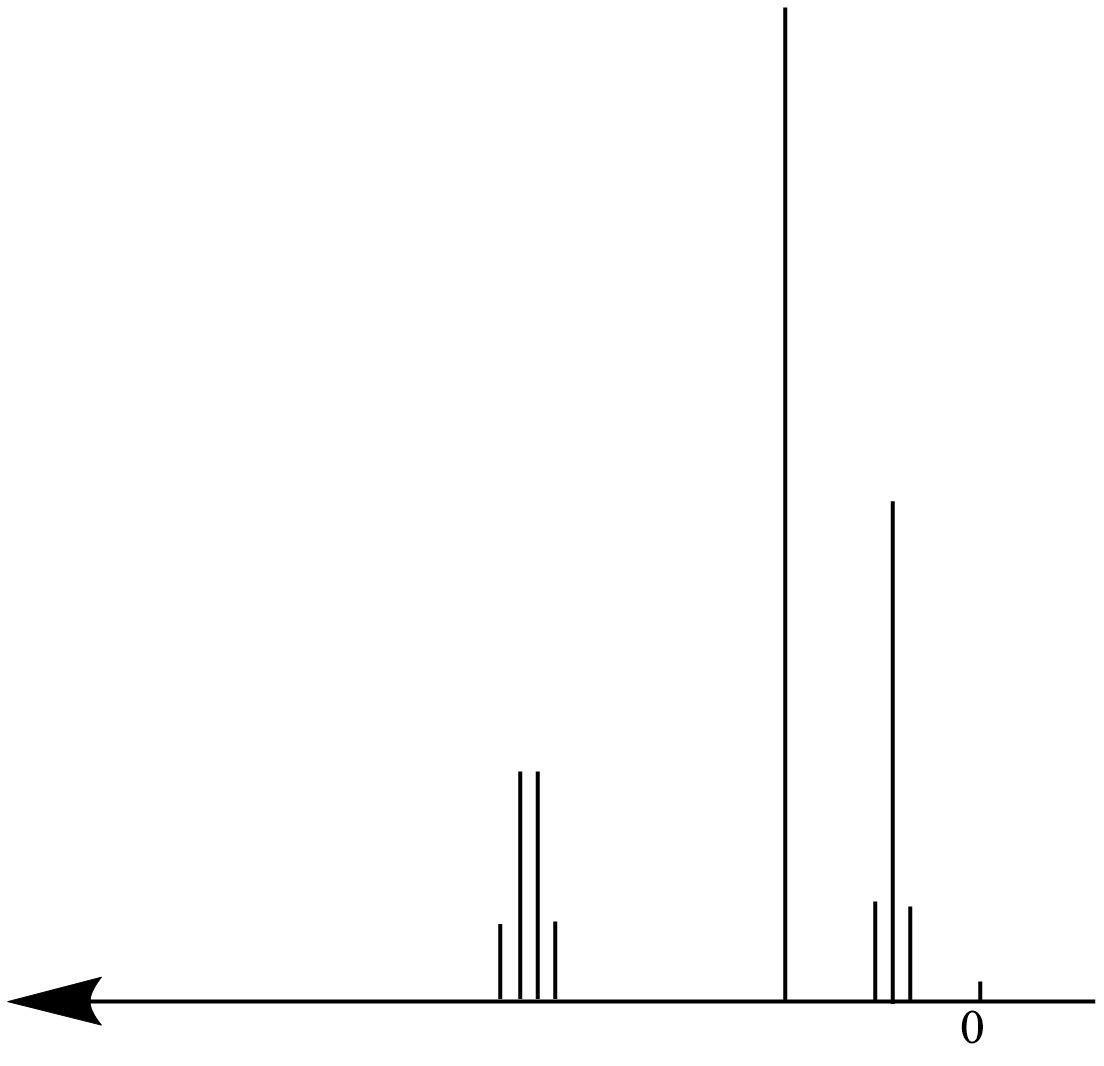
\includegraphics[width=0.4\linewidth]{chap14-14.png}
\end{figure}

\ex{19}
\begin{align}
\hI_+\hI_- &= (\hI_x + \I\hI_y)(\hI_x - \I\hI_y) \notag\\
&= \hI_x^2 + \hI_y^2 - \I[\hI_x,\hI_y] \ntg
&= \hI^2 - \hI_z^2 + \hbar\hI_z
\end{align}
\begin{align}
\hI_-\hI_+ &= (\hI_x - \I\hI_y)(\hI_x + \I\hI_y) \ntg
&= \hI_x^2 + \hI_y^2 + \I[\hI_x,\hI_y] \ntg
&= \hI^2 - \hI_z^2 - \hbar\hI_z
\end{align}

\ex{23}
\begin{align}
E_j = E_j^{(0)} + H_{jj}^{(1)} = E_i^{(0)} + H_{x,jj}^{(1)} + H_{y,jj}^{(1)} + H_{z,jj}^{(1)} 
\end{align}
Since
\begin{align}
E_1^{(0)} &= -\gamma B_0\qty(1 - \dfrac{\sigma_1 + \sigma_2}{2}) \\
E_2^{(0)} &= -\gamma B_0(\sigma_1 - \sigma_2) \\
E_3^{(0)} &= \gamma B_0(\sigma_1 - \sigma_2) \\
E_4^{(0)} &= \gamma B_0\qty(1 - \dfrac{\sigma_1 + \sigma_2}{2}) 
\end{align}
and
\begin{align}
H_{x,jj}^{(1)} &= H_{y,jj}^{(1)} = 0\\
H_{z,11}^{(1)} &= H_{z,44}^{(1)} = \dfrac{hJ_{12}}{4}\\
H_{z,22}^{(1)} &= H_{z,33}^{(1)} = -\dfrac{hJ_{12}}{4}
\end{align}
we have
\begin{align}
E_1 &= -h\nu_0\qty(1 - \dfrac{\sigma_1 + \sigma_2}{2}) + \dfrac{h J_{12}}{4} \\
E_2 &= -h\nu_0(\sigma_1 - \sigma_2) - \dfrac{h J_{12}}{4}\\
E_3 &= h\nu_0(\sigma_1 - \sigma_2) - \dfrac{h J_{12}}{4} \\
E_4 &= h\nu_0\qty(1 - \dfrac{\sigma_1 + \sigma_2}{2}) + \dfrac{h J_{12}}{4}
\end{align}

\ex{30}
\begin{align}
H_{44} &= -\hbar\gamma B_0\Braket{\beta(1)\beta(2) | (1-\sigma_1)\hI_{z1} + (1-\sigma_2)\hI_{z2} | \beta(1)\beta(2)} 
+ \dfrac{hJ_{12}}{\hbar^2}\Braket{\beta(1)\beta(2) | \hI_1\cdot\hI_2 | \beta(1)\beta(2)} \ntg
&= -\gamma B_0[(1-\sigma_1) + (1-\sigma_2)]\qty(-\dfrac{\hbar}{2}) + \dfrac{hJ_{12}}{\hbar^2}\dfrac{\hbar^2}{4} \ntg
&= \dfrac{h\nu_0}{2}[(1-\sigma_1) + (1-\sigma_2)] + \dfrac{hJ_{12}}{4}
\end{align}

\ex{34}
\begin{align}
E_2 - E_1 &= -\dfrac{hJ}{4} 
- \dfrac{h}{2}\sqrt{\nu_0^2(\sigma_1-\sigma_2)^2 + J^2} 
+ h\nu_0\qty(1 - \dfrac{\sigma_1+\sigma_2}{2}) - \dfrac{hJ}{4} \ntg
&= -\dfrac{hJ}{2} - \dfrac{h}{2}\sqrt{\nu_0^2(\sigma_1-\sigma_2)^2 + J^2} 
+ \dfrac{h\nu_0}{2}(2 - \sigma_1 - \sigma_2)
\end{align}
thus
\begin{equation}\label{key}
\nu_{1\ra 2} = \dfrac{E_2 - E_1}{h} = -\dfrac{J}{2} - \dfrac{1}{2}\sqrt{\nu_0^2(\sigma_1-\sigma_2)^2 + J^2} 
+ \dfrac{\nu_0}{2}(2 - \sigma_1 - \sigma_2)
\end{equation}

\ex{36}
~\\$ \bullet $ For $ \nu_0 = \SI{60}{MHz} $,
\begin{align}
\sqrt{\nu_0^2(\sigma_1-\sigma_2)^2 + J^2} = \sqrt{60^2\cross 0.12^2 + 8.0^2} = \SI{10.76}{Hz}
\end{align}
$ \therefore $
\begin{align}
\nu_{1\ra 2} &= \SI{60}{MHz} - \dfrac{1}{2}(8 + 10.76)\si{Hz} = \SI{60}{MHz} - \SI{9.38}{Hz} \\
\nu_{1\ra 3} &= \SI{60}{MHz} - \dfrac{1}{2}(8 - 10.76)\si{Hz} = \SI{60}{MHz} + \SI{1.38}{Hz} \\
\nu_{2\ra 4} &= \SI{60}{MHz} + \dfrac{1}{2}(8 + 10.76)\si{Hz} = \SI{60}{MHz} + \SI{9.38}{Hz} \\
\nu_{3\ra 4} &= \SI{60}{MHz} + \dfrac{1}{2}(8 - 10.76)\si{Hz} = \SI{60}{MHz} - \SI{1.38}{Hz} \\
\end{align}
the relative intensity
\begin{equation}\label{key}
r = 2.25
\end{equation}
\begin{equation}\label{key}
\dfrac{(r-1)^2}{(r+1)^2} = 0.15
\end{equation}

$ \bullet $ For $ \nu_0 = \SI{500}{MHz} $,
\begin{align}
\sqrt{\nu_0^2(\sigma_1-\sigma_2)^2 + J^2} = \sqrt{500^2\cross 0.12^2 + 8.0^2} = \SI{60.5}{Hz}
\end{align}
$ \therefore $
\begin{align}
\nu_{1\ra 2} &= \SI{500}{MHz} - \dfrac{1}{2}(8 + 60.5)\si{Hz} = \SI{60}{MHz} - \SI{34.2}{Hz} \\
\nu_{1\ra 3} &= \SI{500}{MHz} - \dfrac{1}{2}(8 - 60.5)\si{Hz} = \SI{60}{MHz} + \SI{26.2}{Hz} \\
\nu_{2\ra 4} &= \SI{500}{MHz} + \dfrac{1}{2}(8 + 60.5)\si{Hz} = \SI{60}{MHz} + \SI{34.2}{Hz} \\
\nu_{3\ra 4} &= \SI{500}{MHz} + \dfrac{1}{2}(8 - 60.5)\si{Hz} = \SI{60}{MHz} - \SI{26.2}{Hz} \\
\end{align}
the relative intensity
\begin{equation}\label{key}
r = 15.52
\end{equation}
\begin{equation}\label{key}
\dfrac{(r-1)^2}{(r+1)^2} = 0.77
\end{equation}

\ex{39}
The spin functions are
\begin{align}
\phi_1 &= \psi_1 = \alpha(1)\alpha(2) \\
\phi_2 &= \dfrac{1}{\sqrt{2}}(\psi_2 - \psi_3) = \dfrac{1}{\sqrt{2}}(\alpha(1)\beta(2) - \beta(1)\alpha(2) \\
\phi_3 &= \dfrac{1}{\sqrt{2}}(\psi_2 + \psi_3) = \dfrac{1}{\sqrt{2}}(\alpha(1)\beta(2) + \beta(1)\alpha(2) \\ 
\phi_4 &= \psi_4 = \beta(1)\beta(2)
\end{align}
$ \therefore $(using atomic unit)
\begin{align}
P_{x,12} &= \Braket{\phi_2 | \hI_{x1} + \hI_{x2} | \phi_1} = \Braket{\dfrac{1}{\sqrt{2}}(\psi_2 - \psi_3) | \dfrac{1}{2}(\psi_2 + \psi_3)} = 0\\
P_{y,12} &= \Braket{\phi_2 | \hI_{y1} + \hI_{y2} | \phi_1} = \Braket{\dfrac{1}{\sqrt{2}}(\psi_2 - \psi_3) | \dfrac{\I}{2}(\psi_2 + \psi_3)} = 0\\
P_{x,13} &= \Braket{\phi_3 | \hI_{x1} + \hI_{x2} | \phi_1} = \Braket{\dfrac{1}{\sqrt{2}}(\psi_2 + \psi_3) | \dfrac{1}{2}(\psi_2 + \psi_3)} = \dfrac{1}{\sqrt{2}}\\
P_{y,13} &= \Braket{\phi_3 | \hI_{y1} + \hI_{y2} | \phi_1} = \Braket{\dfrac{1}{\sqrt{2}}(\psi_2 + \psi_3) | \dfrac{\I}{2}(\psi_2 + \psi_3)} = \dfrac{\I}{\sqrt{2}}\\
P_{x,14} &= \Braket{\phi_4 | \hI_{x1} + \hI_{x2} | \phi_1} = \Braket{\psi_4 | \dfrac{1}{2}(\psi_2 + \psi_3)} = 0\\
P_{y,14} &= \Braket{\phi_4 | \hI_{y1} + \hI_{y2} | \phi_1} = \Braket{\psi_4 | \dfrac{\I}{2}(\psi_2 + \psi_3)} = 0\\
P_{x,23} &= \Braket{\phi_3 | \hI_{x1} + \hI_{x2} | \phi_2} = \Braket{\psi_3 | 0} = 0\\
P_{y,23} &= \Braket{\phi_3 | \hI_{y1} + \hI_{y2} | \phi_2} = \Braket{\psi_3 | 0} = 0\\
P_{x,24} &= \Braket{\phi_4 | \hI_{x1} + \hI_{x2} | \phi_2} = \Braket{\psi_4 | 0} = 0\\
P_{y,24} &= \Braket{\phi_4 | \hI_{y1} + \hI_{y2} | \phi_2} = \Braket{\psi_4 | 0} = 0\\
P_{x,34} &= \Braket{\phi_4 | \hI_{x1} + \hI_{x2} | \phi_3} = \Braket{\psi_4 | \dfrac{1}{\sqrt{2}}(\psi_1 + \psi_4)} = \dfrac{1}{\sqrt{2}}\\
P_{y,34} &= \Braket{\phi_4 | \hI_{y1} + \hI_{y2} | \phi_3} = \Braket{\psi_4 | \dfrac{\I}{\sqrt{2}}(\psi_1 + \psi_4)} = \dfrac{\I}{\sqrt{2}}
\end{align}
thus, only $ 1\ra 3 $ and $ 3\ra 4 $ are allowed.

\end{document}